\appendix
\clearpage{\renewcommand{\appendixname}{Anexo}

\chapter{Anexos}\label{anex}

\section{Fases y tareas de la metodología CRISP-DM} \label{anex:fases-crisp}
\begin{figure}[H] %la opción H indica al compilador LaTeX que posicione la figura lo más cerca posible de este lugar.
	\centering
	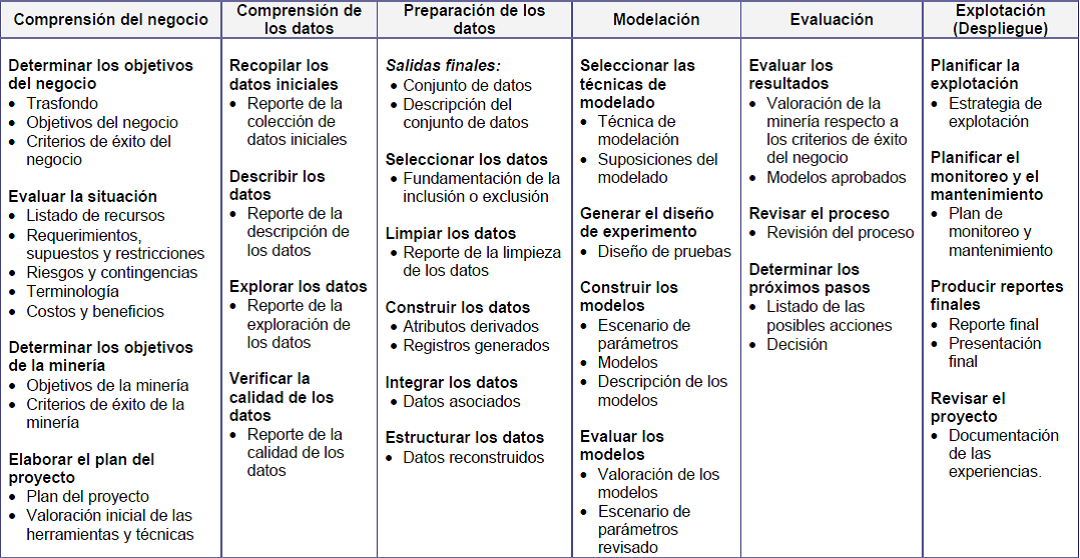
\includegraphics[width=0.95\linewidth]{figuras/fases-crispdm-descritas.png}
	\caption{Fases y tareas de la metodología CRISP-DM.}
	\label{aped.fases-crispdm-descritas} %incluir el label permite referenciarla en cualquier parte del documento.
\end{figure}

\section{Estudio de algoritmos supervisados} \label{anex:estudio-super}
\begin{figure}[H] %la opción H indica al compilador LaTeX que posicione la figura lo más cerca posible de este lugar.
	\centering
	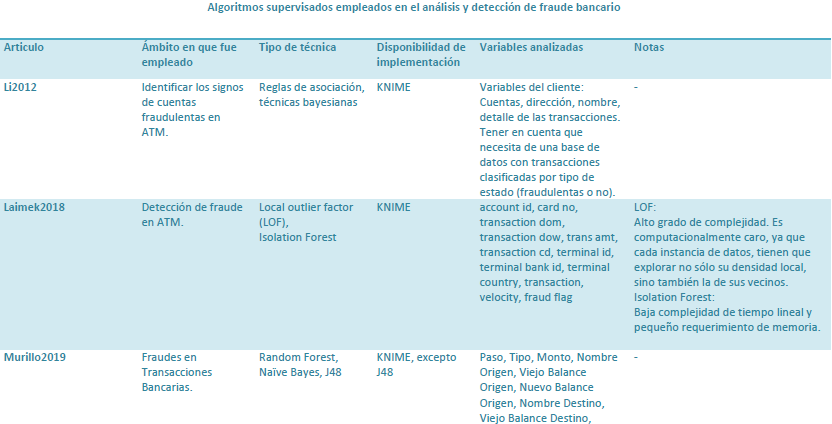
\includegraphics[width=1.0\linewidth]{figuras/superv (1).png}
	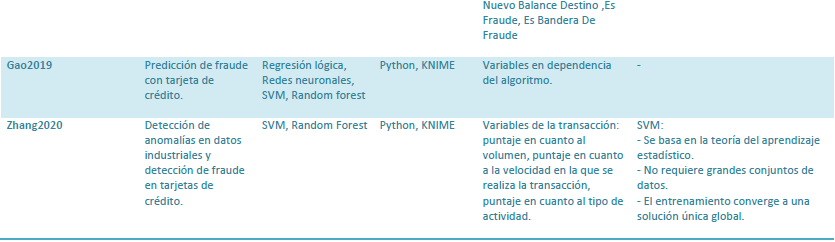
\includegraphics[width=1.0\linewidth]{figuras/superv (2).png}
	\caption{Algoritmos supervisados estudiados dedicados a la detección de fraude bancario}
	\label{aped.supervisados-1} %incluir el label permite referenciarla en cualquier parte del documento.
\end{figure}

\section{Estudio de algoritmos no supervisados} \label{anex:estudio-unsuper}
\begin{figure}[H] %la opción H indica al compilador LaTeX que posicione la figura lo más cerca posible de este lugar.
	\centering
	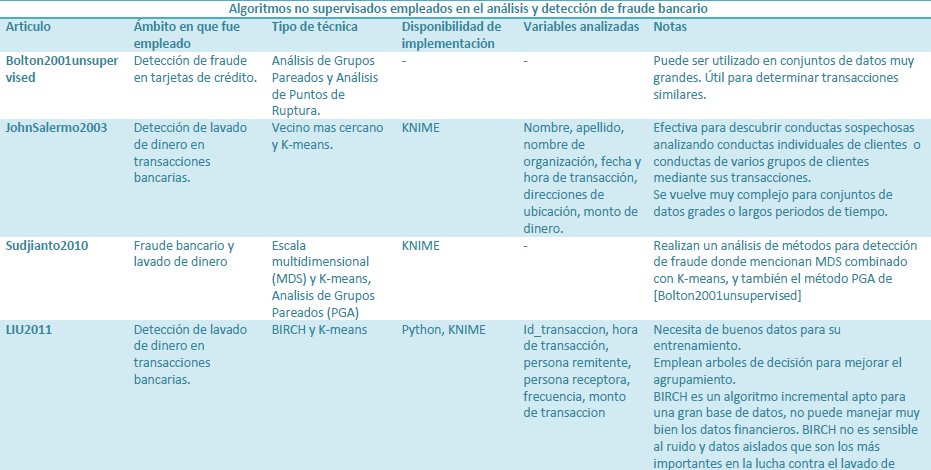
\includegraphics[width=1.0\linewidth]{figuras/no-superv (1).png}
	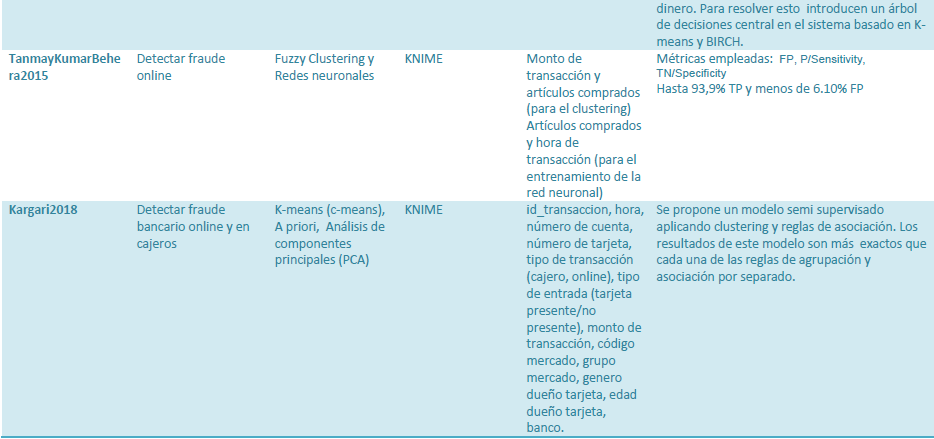
\includegraphics[width=1.0\linewidth]{figuras/no-superv (2).png}
	\caption{Algoritmos no supervisados estudiados dedicados a la detección de fraude bancario}
	\label{aped.no-supervisados-1} %incluir el label permite referenciarla en cualquier parte del documento.
\end{figure}

\section{Modelo de Árbol de Decisión}
	
	\subsection{Resultados de la ejecución del nodo \textit{Decision Tree}} \label{anex:dec-tree-res}

	\begin{figure}[H]
		\centering
		\includegraphics[width=0.8\linewidth]{"figuras/Ray/Arbol de decision/Todas las variables/Histograma"}
		\caption{Resultados del nodo \textit{Decision Tree} con todas las variables de la vista minable}
		\label{aped.hist-all-des-tree}
	\end{figure}

	\begin{figure}[H]
		\centering
		\includegraphics[width=0.8\linewidth]{"figuras/Ray/Arbol de 	decision/Grupo de datos Mejores Resultados/Histograma"}
		\caption{Resultados del nodo \textit{Decision Tree} tras la 	elección de variables}
		\label{aped.hist-mejores-dt}
	\end{figure}

\section{Modelo de Random Forest} \label{random-res}
\subsection{Resultados de la ejecución del nodo \textit{Random Forest}}

\begin{figure} [H]
	\centering
	\includegraphics[width=0.8\linewidth]{"figuras/Ray/Bosque aleatorio/Todas las variables/Histograma"}
	\caption{Resultados del nodo \textit{Random Forest} con todas las variables de la vista minable}
	\label{aped.hist-random-todas}
\end{figure}

\begin{figure}[H]
	\centering
	\includegraphics[width=0.8\linewidth]{"figuras/Ray/Bosque aleatorio/Variables importantes/Grafico de barra"}
	\caption{Resultados del nodo \textit{Random Forest} tras la elección de variables}
	\label{aped.hist-random-best}
\end{figure}



